%%%%%%%%%%%%%%%%%%%%%%
%%%%%%%%%%%%%%%%%%%%%%
\section{Results}
%%%%%%%%%%%%%%%%%%%%%%
%%%%%%%%%%%%%%%%%%%%%%

%%%%%%%%%%%%%%%%%%%%%%
%%%%%%%%%%%%%%%%%%%%%%
\subsection{Performance of individual properties}
%%%%%%%%%%%%%%%%%%%%%%
%%%%%%%%%%%%%%%%%%%%%%
%%%%%%%%%%%%%%%%%%%%%%
%%%%%%%%%%%%%%%%%%%%%%
\subsubsection{SCOP fold}
%%%%%%%%%%%%%%%%%%%%%%
%%%%%%%%%%%%%%%%%%%%%%

\Cref{tab:vqscopt} shows the performance of each property for when predicting SCOP folds.  Among structure based properties we found that $\kappa$ backbone angles had the best performance, both for individual SCOP folds and in terms of its $AUC^{\bf{w}}$ ($0.961$).  Solvent accessibility (SolAcc) values performed the worst out of structure based properties, obtaining the lowest $AUC$ among structure properties for all SCOP folds and in terms of $AUC^{\bf{w}}$ ($0.868$). In general all structure based properties outperformed sequence based properties.  Amongst sequence based properties predicted secondary structures performed the best, especially the predictions that a residue is in a helix ($AUC^{\bf{w}}=0.788$), a loop ($AUC^{\bf{w}}=0.771$), or a sheet ($AUC^{\bf{w}}=0.787$).  Calculated hydrophobicity and VSL2B based predictions of disorder propensity performed the worst ($AUC^{\bf{w}}=0.707$ and $AUC^{\bf{w}}=0.682$ respectively).  As a predictor of disorder PDBDisorder based features performed better than VSL2B ($AUC^{\bf{w}}=0.764$), although this may be based on information leak due to this predictor being trained on PDB data.

 %% TABLE
%%%%%%%%%%%%%%%%%%%%%%
%%%%%%%%%%%%%%%%%%%%%%
\begin{table*}[h]
\resizebox{\columnwidth}{!}{
	\begin{tabular}{|l||rrc|rrc|rrc|rrc||rrc||}
		\hline
		\multirow{2}{*}{Property\textbackslash Category} & \multicolumn{3}{c|}{All $\alpha$}& \multicolumn{3}{c|}{All $\beta$}& \multicolumn{3}{c|}{$\alpha/\beta$}& \multicolumn{3}{c||}{$\alpha+\beta$} & \multicolumn{3}{c||}{$AUC^{\bf{w}}$}\\ 
		\cline{2-16}
		 & $m$ & $n$ & $AUC$ & $m$ & $n$ & $AUC$ & $m$ & $n$ & $AUC$ & $m$ & $n$ & $AUC$ & $m$ & $n$ & $AUC^{\bf{w}}$\\
		\hline
		\hline
		Alpha & 4,096 & 8 & 0.994& 4,096 & 8 & 0.982& 4,096 & 16 & 0.967 & 4,096 & 32 & 0.829 & 4,096 & 8 & 0.930\\
		Kappa & 4,096 & 16 & 0.995& 4,096 & 16 & 0.986& 4,096 & 16 & 0.978 & 4,096 & 32 & 0.903 & 4,096 & 32 & 0.961\\
		Phi & 4,096 & 16 & 0.990& 4,096 & 16 & 0.975& 4,096 & 16 & 0.964 & 4,096 & 32 & 0.809 & 4,096 & 32 & 0.920\\
		Psi & 4,096 & 8 & 0.991& 4,096 & 16 & 0.981& 4,096 & 16 & 0.970 & 4,096 & 32 & 0.850 & 4,096 & 32 & 0.938\\
		SolAcc & 4,096 & 8 & 0.960& 4,096 & 8 & 0.951& 4,096 & 32 & 0.914 & 4,096 & 32 & 0.710 & 4,096 & 32 & 0.868\\
		\hline
		\hline
		B-factors & 256 & 8 & 0.790& 256 & 8 & 0.709& 64 & 8 & 0.809 & 16 & 4 & 0.587 & 64 & 4 & 0.717\\
		Helix & 16 & 4 & 0.868& 16 & 8 & 0.871& 64 & 16 & 0.842 & 64 & 32 & 0.637 & 64 & 32 & 0.788\\
		Hydrophobicity & 256 & 4 & 0.711& 1,024 & 4 & 0.728& 64 & 2 & 0.834 & 64 & 2 & 0.585 & 256 & 4 & 0.707\\
		Loop & 256 & 16 & 0.872& 64 & 8 & 0.848& 16 & 32 & 0.821 & 1,024 & 32 & 0.607 & 64 & 16 & 0.771\\
		PDBDisorder & 1,024 & 8 & 0.842& 64 & 4 & 0.849& 64 & 4 & 0.819 & 256 & 32 & 0.591 & 64 & 4 & 0.764\\
		Sheet & 64 & 2 & 0.904& 64 & 8 & 0.853& 256 & 16 & 0.836 & 64 & 32 & 0.641 & 64 & 32 & 0.787\\
		VSL2B & 16 & 2 & 0.699& 64 & 32 & 0.628& 64 & 8 & 0.812 & 64 & 2 & 0.589 & 64 & 8 & 0.682\\
		\hline
		\hline
		String Kernel & -- & 2 & 0.863& -- & 3 & 0.878& -- & 4 & 0.860& -- & 5 & 0.634 & -- & 4 & 0.794\\
		Sequence  & 64 & 16 & 0.915 & 64 & 16 & 0.876 & 64 & 16 & 0.880 & 64 & 16 & 0.621 & 64 & 16 & 0.813\\
		Structure & 4,096 & 32 & 0.992 & 4,096 & 32 & 0.983 & 4,096 & 32 & 0.979 & 4,096 & 32 & 0.903 & 4,096 & 32 & 0.961\\
		Sequence + Structure & -- & -- & 0.989 & -- & -- & 0.967 & -- & -- & 0.970 & -- & -- & 0.851 & -- & -- & 0.939\\
		Sequence + Structure + SK & -- & -- & 0.989 & -- & -- & 0.967 & -- & -- & 0.970 & -- & -- & 0.851 & -- & -- & 0.939\\

		\hline
		
	\end{tabular}
}
\caption[Optimal property based feature performance when predicting SCOP fold.]{Optimal performance, according to $AUC$, of each property based feature when predicting SCOP fold.  For each property feature the combination of $m$ and $n$ values that obtained the highest $AUC$ for an individual SCOP fold are reported.  The last three columns show the weighted $AUC$, $AUC^{\bf{w}}$, obtained across all SCOP folds. Results when combining all sequence and property based features are shown in the bottom section of the table.  Because different combinations of $m$ and $n$ are used when combining properties these values are not shown for the Sequence + Structure and Sequence + Structure + SK combination of features.}
\label{tab:vqscopt}
\end{table*}

%%%%%%%%%%%%%%%%%%%%%%
%%%%%%%%%%%%%%%%%%%%%%

%%%%%%%%%%%%%%%%%%%%%%
%%%%%%%%%%%%%%%%%%%%%%
\subsubsection{``Catalytic activity"}
%%%%%%%%%%%%%%%%%%%%%%
%%%%%%%%%%%%%%%%%%%%%%
The first column of results in \Cref{tab:vqscopt} show the performance of each property when predicting whether a protein is annotated with the ``catalytic activity" term.  We found that disorder based predictions (VSL2B  $AUC=0.742$ and PDBDisorder $AUC=0.718$) and predicted BFactors ($AUC=0.722$) performed the best, whereas, contrary to their performance in distinguishing between SCOP folds, predicted secondary structures performed the worst (Helix $AUC=0.687$, Loo $AUC=0.698$, and Sheet $AUC=0.681$).

%%%%%%%%%%%%%%%%%%%%%%
%%%%%%%%%%%%%%%%%%%%%%
\subsubsection{``Catalytic activity" subclass}
%%%%%%%%%%%%%%%%%%%%%%
%%%%%%%%%%%%%%%%%%%%%%
\Cref{tab:vqscopt} shows the performance of each property when predicting the tested subclasses of ``catalytic activity".  As with predicting ``catalytic activity," predicted BFactors also performed well in predicting ``catalytic activity" subclass.  ($AUC^{\bf{w}}=0.659$).  Predicted secondary structures had mixed performance, with predicted loops obtaining a comparatively high $AUC^{\bf{w}}$ of $0.647$, whereas helix and sheet predictions only achieved a $AUC^{\bf{w}}$ of $0.511$ and $0.621$ respectively.

%% TABLE
%%%%%%%%%%%%%%%%%%%%%%
%%%%%%%%%%%%%%%%%%%%%%
%\begin{centering}
%\begin{landscape}

%\begin{table*}[htbp]
\clearpage
\begin{sidewaystable}[H]

\vspace*{5in}
\begin{centering}
\resizebox{\textheight}{!}{




		\begin{tabular}{|l||rrc||rrc|rrc|rrc|rrc|rrc|rrc||rrc||}
		\hline
		\multirow{2}{*}{Property\textbackslash Category} & \multicolumn{3}{c||}{catalytic activity} & \multicolumn{3}{c|}{oxidoreductase activity}& \multicolumn{3}{c|}{transferase activity}& \multicolumn{3}{c|}{hydrolase activity}& \multicolumn{3}{c|}{lyase activity}& \multicolumn{3}{c|}{isomerase activity} & \multicolumn{3}{c||}{ligase activity} & \multicolumn{3}{c||}{$AUC^{\bf{w}}$} \\
		\cline{2-25}
		 & $m$ & $n$ & $AUC$ & $m$ & $n$ & $AUC$ & $m$ & $n$ & $AUC$ & $m$ & $n$ & $AUC$ & $m$ & $n$ & $AUC$ & $m$ & $n$ & $AUC$ & $m$ & $n$ & $AUC$ & $m$ & $n$ & $AUC^{\bf{w}}$\\
		\hline
		\hline
		B-factors & 256 & 32 & 0.722 & 4,096 & 32 & 0.709& 4,096 & 32 & 0.644& 4,096 & 32 & 0.630& 4,096 & 4 & 0.688& 4,096 & 32 & 0.738& 4,096 & 32 & 0.671 & -- & -- & 0.659\\
		Helix & 256 & 8 & 0.687 & 4,096 & 8 & 0.634& 4,096 & 32 & 0.603& 4,096 & 32 & 0.600& 4,096 & 32 & 0.644& 4,096 & 32 & 0.665& 4,096 & 8 & 0.595 & -- & -- & 0.611\\
		Hydrophobicity & 4,096 & 2 & 0.701 & 4,096 & 16 & 0.695& 4,096 & 16 & 0.622& 4,096 & 32 & 0.653& 4,096 & 4 & 0.692& 4,096 & 16 & 0.722& 4,096 & 32 & 0.638 & -- & -- & 0.653\\
		Loop & 256 & 32 & 0.698 & 4,096 & 32 & 0.678& 4,096 & 32 & 0.642& 4,096 & 32 & 0.628& 4,096 & 32 & 0.664& 4,096 & 32 & 0.712& 4,096 & 32 & 0.638 & -- & -- & 0.647\\
		PDBDisorder & 256 & 32 & 0.718 & 4,096 & 32 & 0.683& 4,096 & 32 & 0.645& 4,096 & 16 & 0.640& 4,096 & 32 & 0.676& 4,096 & 32 & 0.717& 4,096 & 16 & 0.635 & -- & -- & 0.65\\
		Sheet & 256 & 4 & 0.681 & 4,096 & 32 & 0.651& 4,096 & 32 & 0.612& 4,096 & 32 & 0.606& 4,096 & 32 & 0.649& 4,096 & 32 & 0.683& 1,024 & 32 & 0.611 & -- & -- & 0.621\\
		VSL2B & 256 & 16 & 0.742 & 1,024 & 32 & 0.661& 4,096 & 16 & 0.594& 4,096 & 32 & 0.614& 4,096 & 32 & 0.638& 4,096 & 32 & 0.680& 1,024 & 8 & 0.630 & -- & -- & 0.620\\
		\hline
		\hline
		String Kernel & -- & 5 &0.857 & -- & 5 & 0.949& -- & 6 & 0.928& -- & 6 & 0.934& -- & 6 & 0.929& -- & 5 & 0.920& -- & 5 & 0.910 & -- & -- & 0.930\\


		Combined & 256 & 16 & 0.776 & 4,096 & 32 & 0.805 & 4,096 & 32 & 0.753 & 4,096 & 32 & 0.754 & 4,096 & 32 & 0.779 & 4,096 & 32 & 0.816 & 4,096 & 32 & 0.763 & 4,096 & 32 & 0.767\\
		Combined + SK & -- & -- & 0.781 & -- & -- & 0.805 & -- & -- & 0.753 & -- & -- & 0.754 & -- & -- & 0.779 & -- & -- & 0.816 & -- & -- & 0.763 & -- & -- & 0.767\\
		\hline
		\hline
		%$NR_{40}$ String Kernel & -- & 5 & ca auc & 4,096 & 32 & 0.203 & -- & -- & 0.179 & -- & -- & 0.181 & -- & -- & 0.216 & -- & -- & 0.230 & -- & -- & 0.195 & -- & -- & 0.189\\
		%$NR_{40}$ String Kernel & CA m & CA n & ca auc & -- & -- & 0.712 & -- & -- & 0.663 & -- & -- & 0.718 & -- & -- & 0.711 & -- & -- & 0.733 & -- & -- & 0.636 & -- & -- & 0.694\\

		%$NR_{40}$ Combined & 256 & 16 & ca auc & 4,096 & 32 & 0.299 & 4,096 & 32 & 0.415 & 4,096 & 32 & 0.416 & 4,096 & 32 & 0.207 & 4,096 & 32 & 0.187 & 4,096 & 32& 0.178 & 4,096 & 32& 0.357\\
		%$NR_{40}$ Combined & CA m & CA n & ca auc & -- & -- & 0.622 & -- & -- & 0.583 & -- & -- & 0.600 & -- & -- & 0.612 & -- & -- & 0.602 & -- & -- & 0.548 & -- & -- & 0.596\\

		%$NR_{40}$ Combined + SK & -- & -- & ca auc & -- & -- & 0.273 & -- & -- & 0.397 & -- & -- & 0.394 & -- & -- & 0.205 & -- & -- & 0.188 & -- & -- & 0.179 & -- & -- & 0.340\\
		%$NR_{40}$ Combined + SK & CA m & CA n & ca auc & -- & -- & 0.627 & -- & -- & 0.589 & -- & -- & 0.606 & -- & -- & 0.619 & -- & -- & 0.602 & -- & -- & 0.552 & -- & -- & 0.601\\

		\hline
		\hline
		
		$NR_{40}$ String Kernel & -- & 5 & 0.733 & -- & -- & 0.733 & -- & -- & 0.619 & -- & -- & 0.612 & -- & -- & 0.725 & -- & -- & 0.669 & -- & -- & 0.668 & -- & -- & 0.649\\
		$NR_{40}$ Combined & 256 & 16 & 0.775 & 4,096 & 32 & 0.681 & 4,096 & 32 & 0.560 & 4,096 & 32 & 0.545 & 4,096 & 32 & 0.617 & 4,096 & 32 & 0.641 & 4,096 & 32 & 0.570 & 4,096 & 32 & 0.583\\
		$NR_{40}$ Combined + SK & -- & -- & 0.775 & -- & -- & 0.681 & -- & -- & 0.559 & -- & -- & 0.548 & -- & -- & 0.629 & -- & -- & 0.649 & -- & -- & 0.574 & -- & -- & 0.585\\


		\hline
				
	\end{tabular}
	%\end{minipage}
}

\caption[Optimal property based feature performance when predicting ``catalytic activity" subclass.]{Optimal performance, according to $AUC$, of each property based feature when predicting ``catalytic activity" subclass.  For each property feature the combination of $m$ and $n$ values that obtained the highest $AUC$ for an individual ``catalytic activity" subclass are reported.}

\label{tab:vqgot}

\end{centering}
%\end{table*}
%\end{sideways}
\end{sidewaystable}
%\end{landscape}




%%%%%%%%%%%%%%%%%%%%%%
%%%%%%%%%%%%%%%%%%%%%%

\subsection{Combined kernel performance}

%%%%%%%%%%%%%%%%%%%%%%
%%%%%%%%%%%%%%%%%%%%%%
\subsubsection{SCOP fold}
%%%%%%%%%%%%%%%%%%%%%%
%%%%%%%%%%%%%%%%%%%%%%
%% Figure
%%%%%%%%%%%%%%%%%%%%%%
%%%%%%%%%%%%%%%%%%%%%%
\begin{figure*}[t!]
\begin{centering}
	\begin{subfigure}[b]{0.23\textwidth}
                \centering
                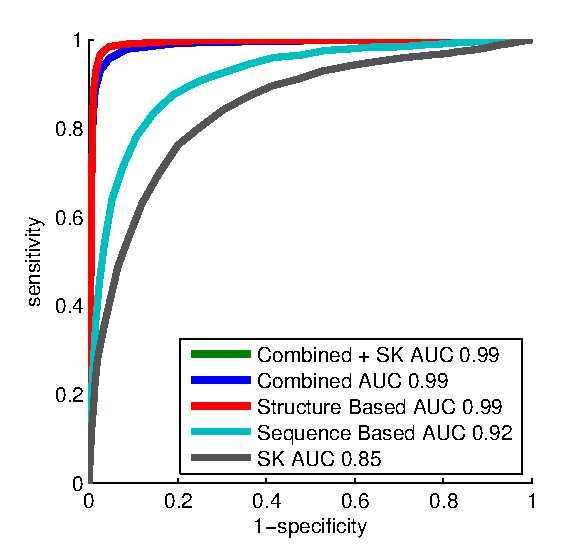
\includegraphics[width=\textwidth]{Figures/vq/SCOP_ROC/all_alpha_ROC}
                \caption{Alll $\alpha$}
                \label{fig:ocS1A}
        \end{subfigure}%
        \quad
	\begin{subfigure}[b]{0.23\textwidth}
                \centering
                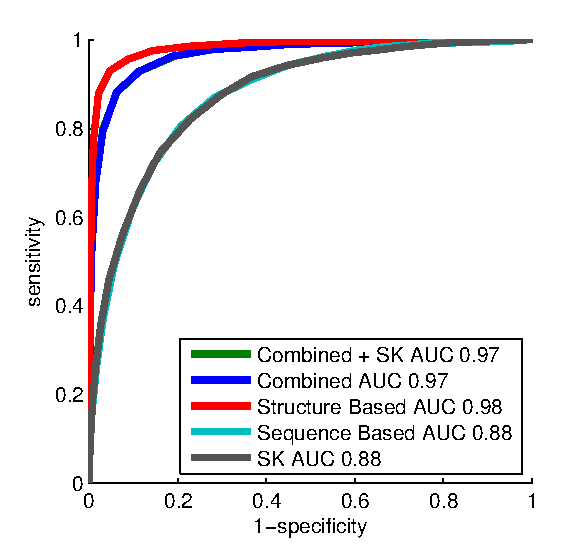
\includegraphics[width=\textwidth]{Figures/vq/SCOP_ROC/all_beta_ROC}
                \caption{All $\beta$}
                \label{fig:ocS1B}
        \end{subfigure}
	\quad
	\begin{subfigure}[b]{0.23\textwidth}
                \centering
                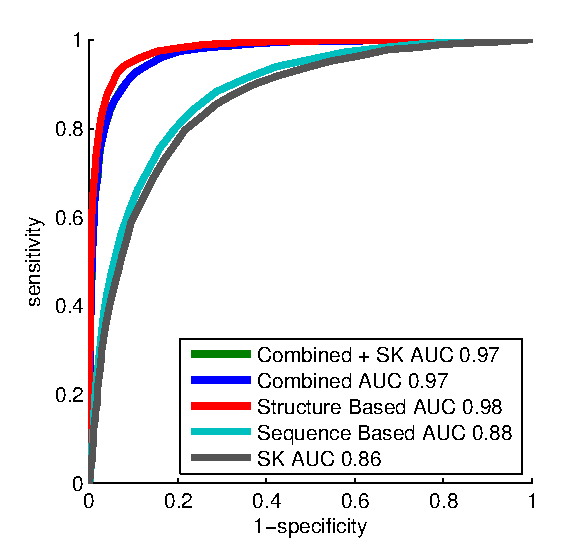
\includegraphics[width=\textwidth]{Figures/vq/SCOP_ROC/alpha_div_beta_ROC}
                \caption{$\alpha$/\ $\beta$}
                \label{fig:ocS1A}
        \end{subfigure}%
        \quad
	\begin{subfigure}[b]{0.23\textwidth}
                \centering
                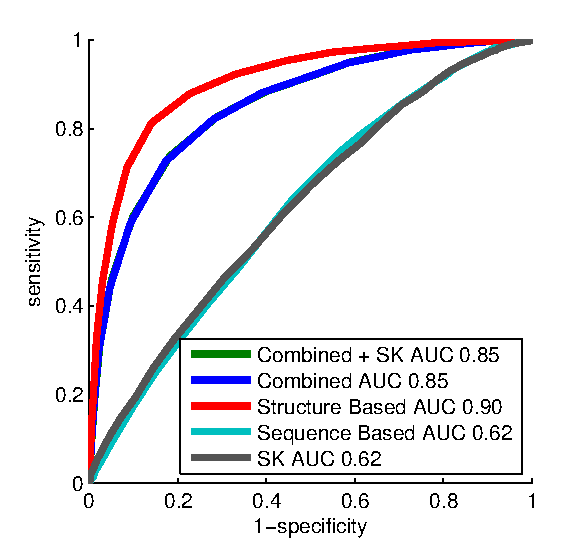
\includegraphics[width=\textwidth]{Figures/vq/SCOP_ROC/alpha_plus_beta_ROC}
                \caption{$\alpha$ + $\beta$}
                \label{fig:ocS1B}
        \end{subfigure}

\end{centering}
\caption[SCOP ROC curves]{SCOP ROC curves showing the performance of each combination of combined features and the string kernel when predicting each category of SCOP fold tested.}
\label{fig:SCOP_ROC}
\end{figure*}




%%%%%%%%%%%%%%%%%%%%%%
%%%%%%%%%%%%%%%%%%%%%%

%\begin{figure*}[t!]
%\begin{centering}
%	\begin{subfigure}[b]{0.35\textwidth}
%                \centering
%                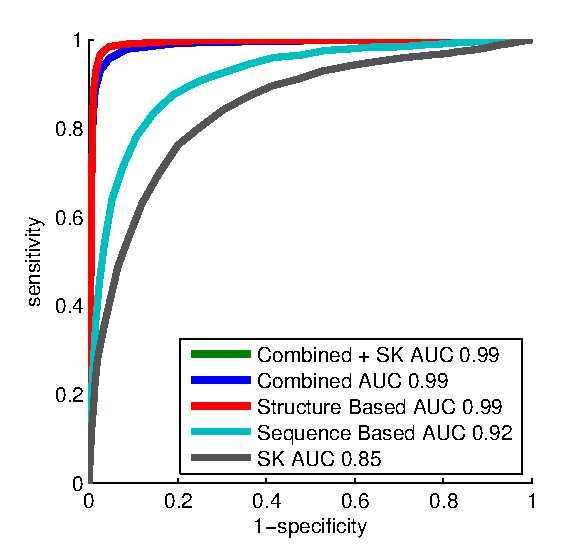
\includegraphics[width=\textwidth]{Figures/vq/SCOP_ROC/all_alpha_ROC}
%                \caption{Alll $\alpha$}
%                \label{fig:ocS1A}
%        \end{subfigure}%
%        \quad
%        \quad
%        \quad
%	\begin{subfigure}[b]{0.35\textwidth}
%                \centering
%                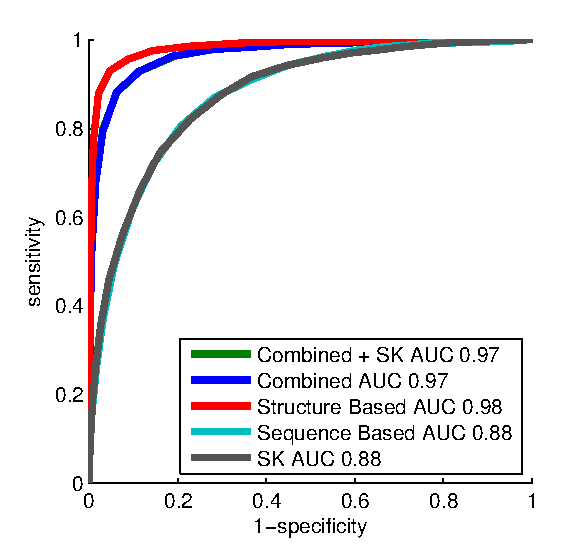
\includegraphics[width=\textwidth]{Figures/vq/SCOP_ROC/all_beta_ROC}
%                \caption{All $\beta$}
%                \label{fig:ocS1B}
%        \end{subfigure}
%
%	\begin{subfigure}[b]{0.35\textwidth}
%                \centering
%                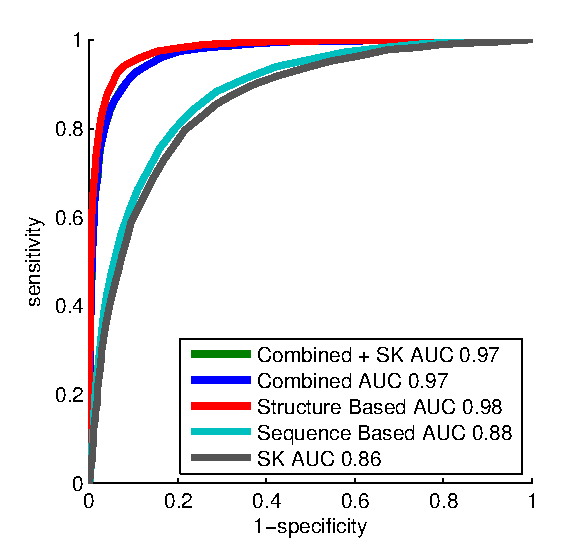
\includegraphics[width=\textwidth]{Figures/vq/SCOP_ROC/alpha_div_beta_ROC}
%                \caption{$\alpha$/\ $\beta$}
%                \label{fig:ocS1A}
%        \end{subfigure}%
%        \quad
%        \quad
%        \quad
%	\begin{subfigure}[b]{0.35\textwidth}
%                \centering
%                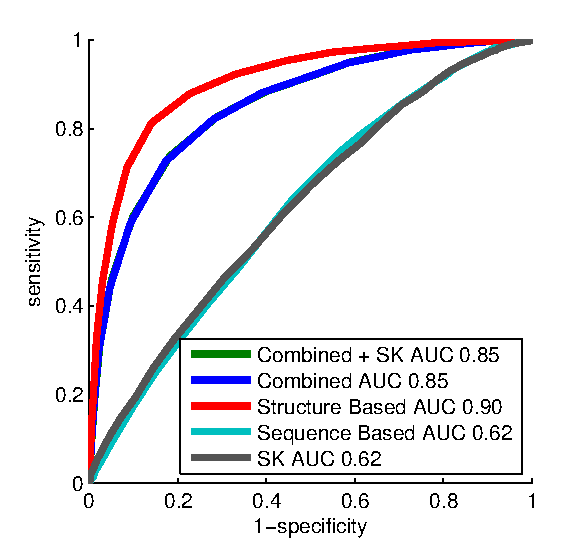
\includegraphics[width=\textwidth]{Figures/vq/SCOP_ROC/alpha_plus_beta_ROC}
%                \caption{$\alpha$ + $\beta$}
%                \label{fig:ocS1B}
%        \end{subfigure}
%
%\end{centering}
%\caption[SCOP ROC Curves]{SCOP ROC Curves showing the performance of each combination of combined features and the string kernel when predicting each category of SCOP fold tested.}
%\label{fig:SCOP_ROC}
%\end{figure*}

%%%%%%%%%%%%%%%%%%%%%%
%%%%%%%%%%%%%%%%%%%%%%
%%%%%%%%%%%%%%%%%%%%%%
%%%%%%%%%%%%%%%%%%%%%%

%%%%%%%%%%%%%%%%%%%%%%
%%%%%%%%%%%%%%%%%%%%%%
\subsubsection{``Catalytic activity"}
%%%%%%%%%%%%%%%%%%%%%%
%%%%%%%%%%%%%%%%%%%%%%

%%%%%%%%%%%%%%%%%%%%%%
%%%%%%%%%%%%%%%%%%%%%%
\subsubsection{``Catalytic activity" subclass}
%%%%%%%%%%%%%%%%%%%%%%
%%%%%%%%%%%%%%%%%%%%%%

%% Figure
%%%%%%%%%%%%%%%%%%%%%%
%%%%%%%%%%%%%%%%%%%%%%
%%%%%%%%%%%%%%%%%%%%%%
%%%%%%%%%%%%%%%%%%%%%%

\begin{figure*}[t!]
\begin{centering}
	\begin{subfigure}[b]{0.25\textwidth}
                \centering
                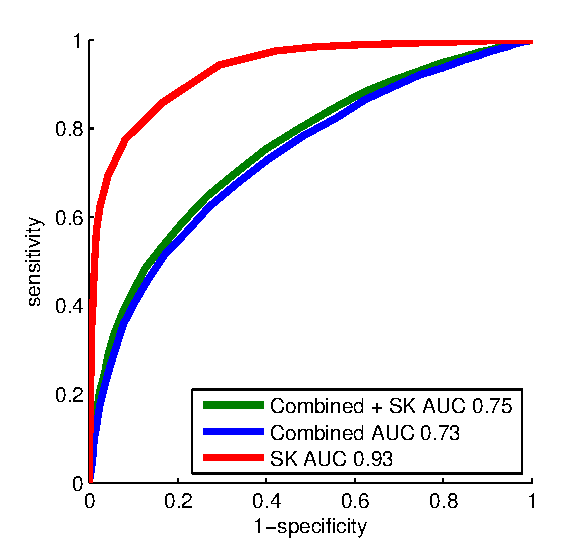
\includegraphics[width=\textwidth]{Figures/vq/GO_SC_ROC/hydrolase_activity_ROC}
                \caption{hydrolase activity}
                \label{fig:hydrolase_activity_ROC}
        \end{subfigure}%
        \quad
	\begin{subfigure}[b]{0.25\textwidth}
                \centering
                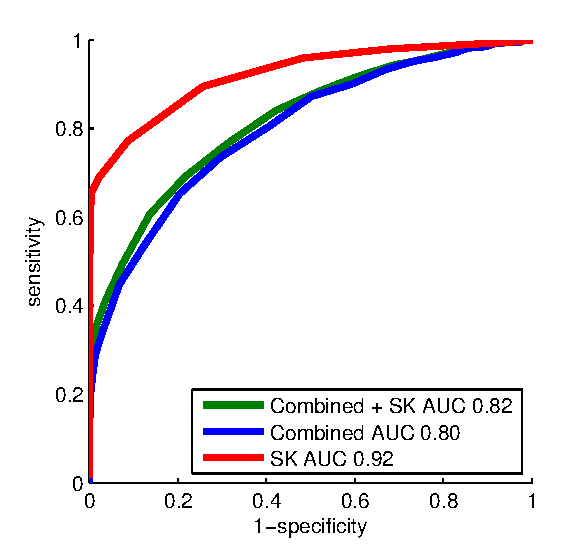
\includegraphics[width=\textwidth]{Figures/vq/GO_SC_ROC/isomerase_activity_ROC}
                \caption{isomerase activity}
                \label{fig:isomerase_activity_ROC}
        \end{subfigure}
        \quad
	\begin{subfigure}[b]{0.25\textwidth}
                \centering
                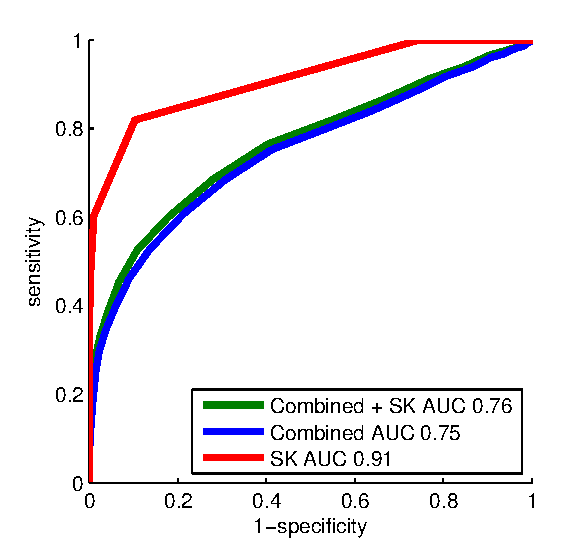
\includegraphics[width=\textwidth]{Figures/vq/GO_SC_ROC/ligase_activity_ROC}
                \caption{ligase activity}
                \label{fig:ligase_activity_ROC}
        \end{subfigure}

	\begin{subfigure}[b]{0.25\textwidth}
                \centering
                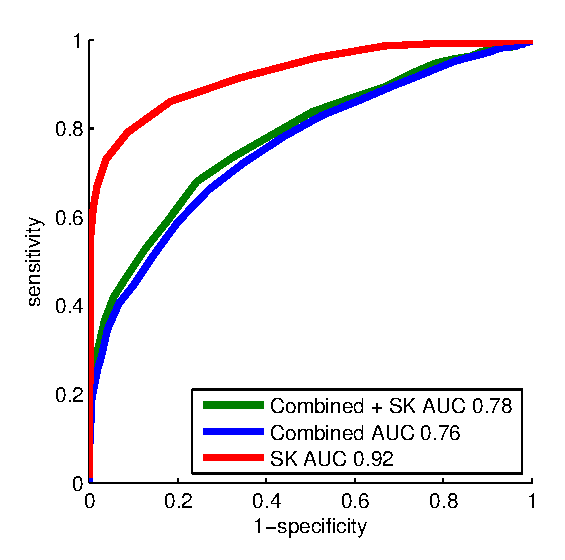
\includegraphics[width=\textwidth]{Figures/vq/GO_SC_ROC/lyase_activity_ROC}
                \caption{lyase activity}
                \label{fig:lyase_activity_ROC}
        \end{subfigure}%
        \quad
	\begin{subfigure}[b]{0.25\textwidth}
                \centering
                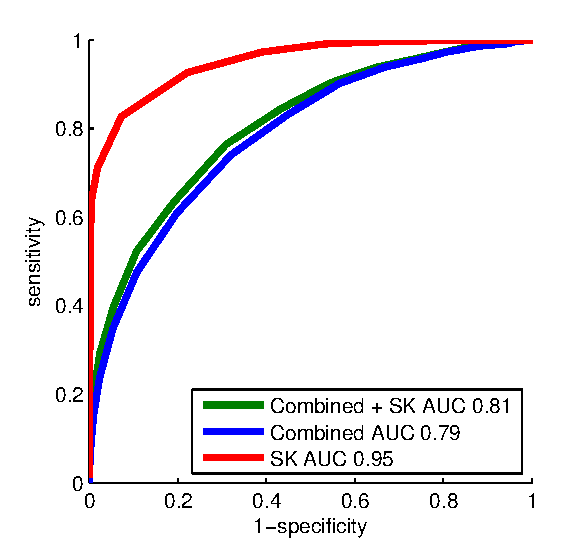
\includegraphics[width=\textwidth]{Figures/vq/GO_SC_ROC/oxidoreductase_activity_ROC}
                \caption{oxidoreductase activity}
                \label{fig:oxidoreductase_activity_ROC}
        \end{subfigure}
        \quad
	\begin{subfigure}[b]{0.25\textwidth}
                \centering
                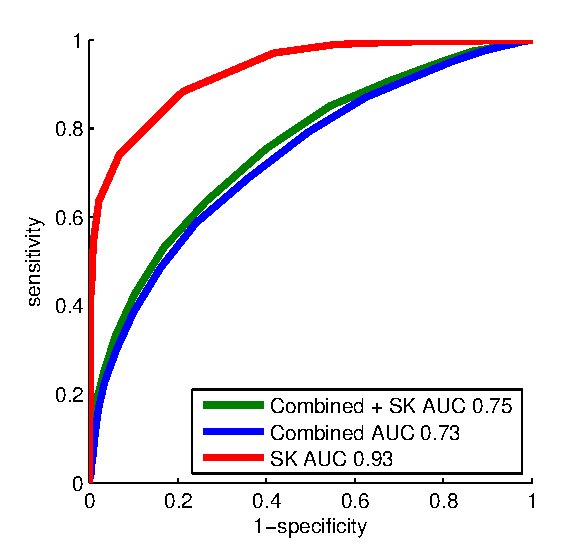
\includegraphics[width=\textwidth]{Figures/vq/GO_SC_ROC/transferase_activity_ROC}
                \caption{transferase activity}
                \label{fig:transferase_activity_ROC}
        \end{subfigure}

\end{centering}
\caption[``catalytic activity" subclass ROC curves]{ROC curves when showing the performance of each combination of combined features and the string kernel when predicting each subclass of ``catalytic activity".}
\label{fig:GO_SC_ROC}
\end{figure*}

%%%%%%%%%%%%%%%%%%%%%%
%%%%%%%%%%%%%%%%%%%%%%
%%%%%%%%%%%%%%%%%%%%%%
%%%%%%%%%%%%%%%%%%%%%%


%%%%%%%%%%%%%%%%%%%%%%
%%%%%%%%%%%%%%%%%%%%%%
%\afterpage{
%\begin{figure*}[t!htpb]
%\begin{centering}
%
%	\begin{subfigure}[b]{0.75\textwidth}
%                \centering
%                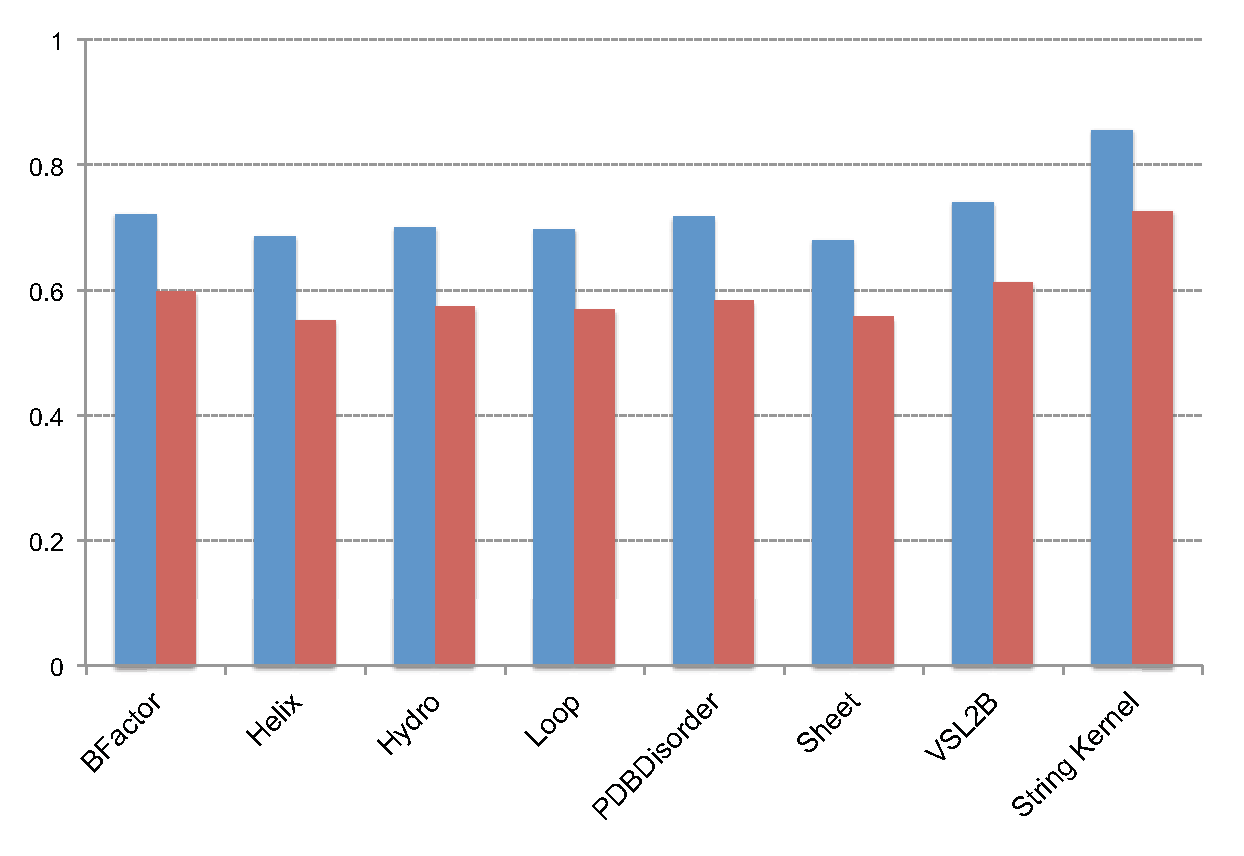
\includegraphics[width=\textwidth]{Figures/vq/count_kernel/GO_Enzyme_Bar}
%                \caption{Catalytic activity}
%                \label{fig:vqresults1B}
%        \end{subfigure}%
%\quad
%	\begin{subfigure}[b]{0.75\textwidth}
%                \centering
%                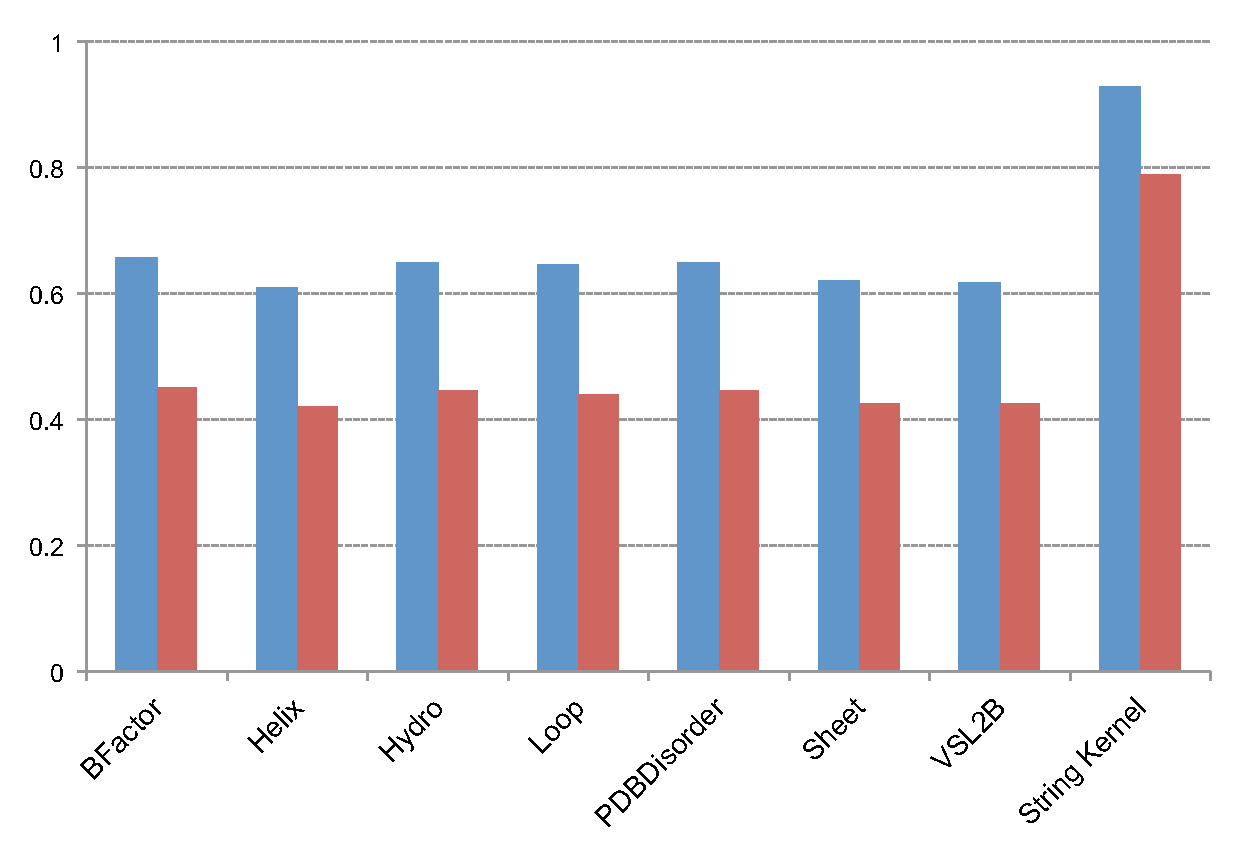
\includegraphics[width=\textwidth]{Figures/vq/count_kernel/GO_SC_Bar}
%                \caption{Catalytic activity subclass}
%                \label{fig:vqresults1C}
%        \end{subfigure}%
%
%
%\par\end{centering}
%\caption[Count kernel individual feature performance]{A bar chart showing the $AUC$ (blue) and $F_{\max}$ (red) performance of individual features in the task of GO function prediction.  Only the best performing combinations of $m$ and $n$ for an individual feature according to $AUC$ or $F_{\max}$ are reported.  Results are shown for the task of predicting  ``catalytic activity" GO term (\Cref{fig:vqresults1B}), and ``catalytic activity" subclass (\Cref{fig:vqresults1C}).  }
%\label{fig:vqresults1}
%\end{figure*}
%}
%%%%%%%%%%%%%%%%%%%%%%
%%%%%%%%%%%%%%%%%%%%%%
%%%%%%%%%%%%%%%%%%%%%%
%%%%%%%%%%%%%%%%%%%%%%
%\begin{figure*}[h!]
%\begin{centering}
%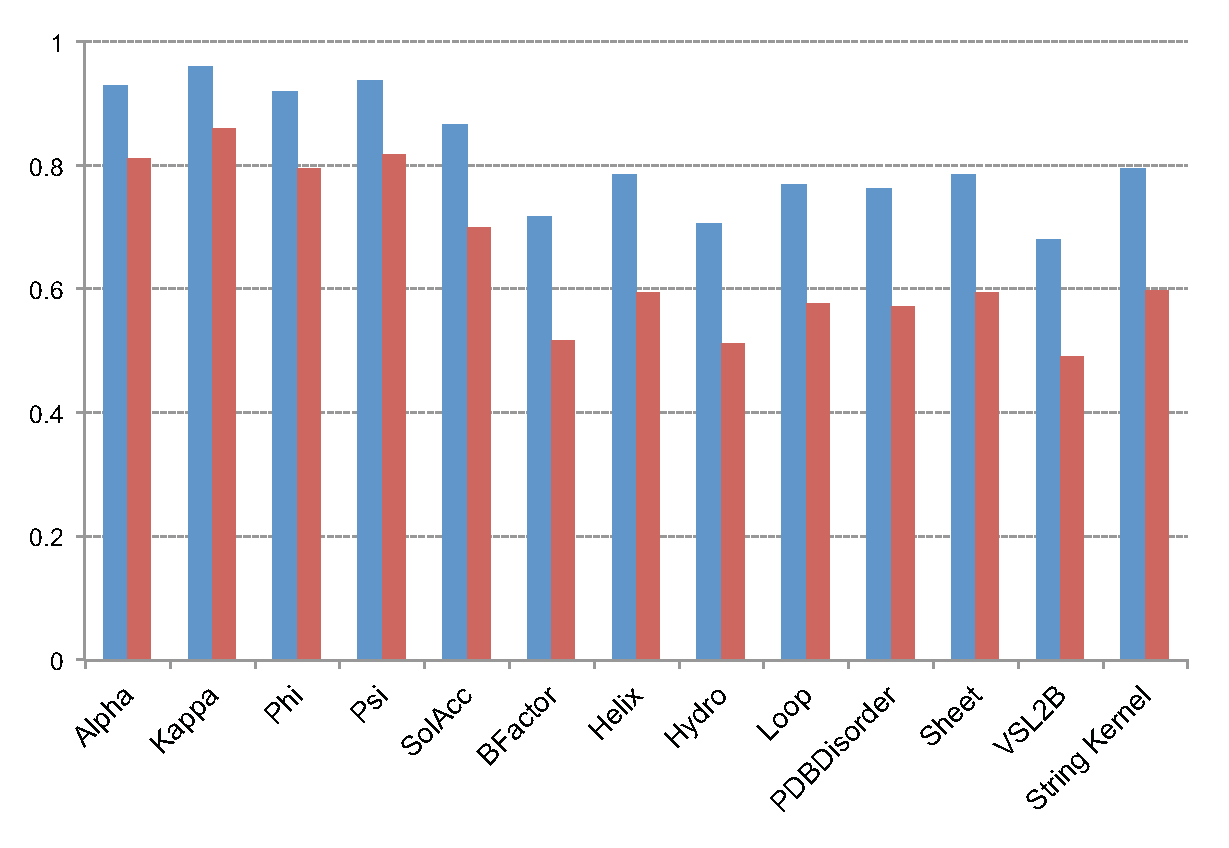
\includegraphics[width=.75\textwidth]{Figures/vq/count_kernel/SCOP_Bar}
%\par\end{centering}
%\caption[Count based kernel performance predicting SCOP fold]{A bar chart showing the $AUC$ (blue) and $F_{\max}$ (red) performance of individual features. Only the best performing combinations of $m$ and $n$ for an individual feature according to $AUC$ or $F_{\max}$ are reported. }
%\label{fig:vqscopcount}
%\end{figure*}
%%%%%%%%%%%%%%%%%%%%%%
%%%%%%%%%%%%%%%%%%%%%%


%%%%%%%%%%%%%%%%%%%%%%%
%%%%%%%%%%%%%%%%%%%%%%%
%\subsection{Agreement of $AUC$ and $F_{\max}$}
%%%%%%%%%%%%%%%%%%%%%%%
%%%%%%%%%%%%%%%%%%%%%%%
%
%Looking at \Cref{tab:vqgostandardperformance,tab:vqscopstandardperformance} we found strong agreement in the values of $m$ and $n$ at which each feature type achieved its maximum $AUC$ and $F_{\max}$ values for the count based kernel, especially for the prediction of SCOP fold and ``catalytic activity" subclass.  While agreement wasn't as strong for the prediction of ``catalytic activity," differences in optimal $m$ and $n$ values were not drastic; the most notable of which were those determined for the hydrophobicity property feature where $AUC$ found that $m=4096, n=2$ was optimal whereas $F_{\max}$ found that $m=256, n=32$ was optimal.  
%
%%There was noticeably less agreement between optimal $m$ and $n$ values designated by $AUC$ and $F_{\max}$ when looking at the similarity augmented count kernel, with the $F_{\max}$ value seeming to favor smaller numbers of centroids for structure based features.  While there is little agreement between these metrics for the similarity augmented count kernel this may be due to the poor overall performance of this kernel.
%%
%%Although the sample size for determining agreement in optimal $m$ and $n$ values is smaller for the additive kernel because it was only fully tested on the hydrophobicity sequence property, there are multiple alpha values at which optimal $m$ and $n$ values can be compared.